\section{Ornstein-Uhlenbeck Processes}

The Ornstein-Uhlenbeck process $(X_t : t \ge 0)$ is a diffusion process on $\mbb{R}$ with generator 
$$
(\mathcal{L}f)(x) = - \alpha x f'(x) + \frac{1}{2}\sigma^2 f''(x)
$$
with $\alpha,\,\sigma^2 > 0$, and we consider a fixed initial condition $X_0 = x_0$.

\begin{enumerate}
    \item[(a)] Use the evolution equation of expectation values of test functions $f: \mathbb{R} \to \mathbb{R}$
    \begin{equation}\label{eqn11}
        \frac{\dif}{\dif t} \mbb{E} [f(X_t)]  = \mbb{E} [\mathcal{L}f(X_t)],
    \end{equation}
    to derive ODEs for the mean $m(t):=\mbb{E}[X_t]$ and the variance $v(t) := \mbb{E}[X_t^2] - m(t)^2$, and solve them.

    \textit{ Sol. } Set $f(x) = x$ in the evolution equation \eqref{eqn11}, then we have 
    \begin{equation*}
        \frac{\dif}{\dif t} \mbb{E} [X_t]  = \mbb{E} [\mathcal{L}f(X_t)] = \mbb{E} [- \alpha X_t] = -\alpha \mbb{E} [X_t],
    \end{equation*}
    which is 
    \begin{equation}\label{eqn12}
        \frac{\dif m(t)}{\dif t} = - \alpha m(t)
    \end{equation}
    The general solution to \eqref{eqn12} is 
    \begin{equation*}
        m(t) = C \cdot e^{-\alpha t},
    \end{equation*}
    where $C \in \mbb{R}$ is a constant. By $m(0) = \mbb{E}[X_0] = \mbb{E}[x_0] = x_0$, we know $C = x_0$. Thus, the solution to \eqref{eqn12} is 
    \begin{equation}
        m(t) = x_0 \cdot e^{-\alpha t}.
    \end{equation}

    Setting $f(x) = x^2$ in \eqref{eqn11} gives 
    \begin{align}
        \frac{\dif}{\dif t} \mbb{E}[X_t^2] = & \mbb{E} [ - \alpha X_t \cdot 2X_t + \frac{1}{2}\sigma^2 \cdot 2] \notag \\ 
        = & \mbb{E} [ -2 \alpha X_t^2 + \sigma^2] \notag \\ 
        = & -2 \alpha \mbb{E} [X_t^2] + \sigma^2 \label{eqn13}
    \end{align}
    To solve \eqref{eqn13}, we need to find the general solution $h(t)$ of its homogeneous version and a pariticular solution $p(t)$ of it separatively. So $h(t)$ satisfies 
    \begin{equation*}
        \frac{\dif h(t)}{\dif t} = -2 \alpha h(t).
    \end{equation*}
    Using the method of separation of variables again, we know $h(t) = C_1 \cdot e^{-2\alpha t}$, where $C_1 \in \mbb{R}$ is a constant. 

    Now suppose $p(t) = e^{-2\alpha t} + C_2$ with $C_2 \in \mbb{R}$ being a constant. Then we have
    \begin{align*}
        \frac{\dif p(t)}{\dif t} = & -2 \alpha p(t) + \sigma^2 \\ 
        -2 \alpha e^{-2 \alpha t} = & -2 \alpha (e^{-2\alpha t} + C_2 ) + \sigma^2 \\ 
        2 \alpha C_2 = & \sigma^2 \\ 
        C_2 = & \frac{\sigma^2}{2\alpha}.
    \end{align*}
    So a particular solution $p(t)$ is $p(t) = e^{-2\alpha t} +  \frac{\sigma^2}{2\alpha}$.

    Thus, the general solution of \eqref{eqn13} is $\mbb{E} [X_t^2] = C_1 \cdot e^{-2\alpha t} +  \frac{\sigma^2}{2\alpha}$. By $\mbb{E} [X_0^2] = \mbb{E} [x_0^2] = x_0^2$, we have $C_1 = x_0^2 - \frac{\sigma^2}{2\alpha}$. So the second central moment of $X_t$ is 
    $$\mbb{E}[X_t^2] = \left( x_0^2 - \frac{\sigma^2}{2\alpha} \right) e^{-2\alpha t} + \frac{\sigma^2}{2\alpha},$$
    and the variance of $X_t$ is 
    \begin{align*}
        v(t) = & \mbb{E} [X_t^2] - (\mbb{E}[X_t])^2 \\ 
        = &  \left( x_0^2 - \frac{\sigma^2}{2\alpha} \right) e^{-2\alpha t} + \frac{\sigma^2}{2\alpha} - \left( x_0 \cdot e^{-\alpha t} \right)^2 \\ 
        = &  \frac{\sigma^2}{2 \alpha} \cdot \left(1- e^{-2\alpha t} \right).
    \end{align*}

    \item[(b)] Using the fact that $(X_t: t\ge 0)$ is a Gaussian process, give the distribution of $X_t$ for all $t \ge 0$. 
    
    What is the stationary distribution of the process?

    \textit{ Sol. } In (a), we have solved $\mbb{E}[X_t]$ and $\mbb{VAR}[X_t]$:
    $$
    \mbb{E}[X_t] = m(t) = x_0 \cdot e^{-\alpha t} \quad \text{and} \quad \mbb{VAR}[X_t] = v(t) = \frac{\sigma^2}{2 \alpha} \cdot \left(1- e^{-2\alpha t} \right).
    $$
    Since the process $(X_t: t \ge 0)$ is a Gaussian process, we know $X_t$ follows a Gaussian distribution. Thus, 
    $$
    X_t \sim \mathcal{N}\left( x_0 \cdot e^{-\alpha t}, \, \frac{\sigma^2}{2 \alpha} \cdot \left(1- e^{-2\alpha t} \right) \right).
    $$

    From lecture, we know the stationary density of the diffusion process with time-independent $a(y) \in \mbb{R}$ and $\sigma^2(y) > 0$ has the unnormalized stationary density
    $$
    p(x) = \exp\left(\int_0^x \frac{2a(y) - (\sigma^2)'(y)}{\sigma^2(y)} \dif y \right).
    $$
    Since the Ornstein-Uhlenbeck process is a special case of the diffusion process with $a(y) = -\alpha y$ and $\sigma^2(y) = \sigma^2$, we know the unnormalized stationary density of the Ornstein-Uhlenbeck process is 
    \begin{align*}
        p(x) = & \exp\left(\int_0^x \frac{- 2 \alpha y - 0}{\sigma^2} \dif y \right) \\ 
        = & \exp \left(- \frac{\alpha x^2}{\sigma^2} \right) \\ 
        = & \exp \left( - \frac{ (x - 0)^2}{2 \cdot \frac{\sigma^2}{2\alpha} } \right).
    \end{align*}
    So the stationary distribution of the process is $\mathcal{N}(0, \frac{\sigma^2}{2\alpha})$.

    \item[(c)] For $\alpha = 1$, $\sigma^2 = 1$ and $x_0 = 5$, simulate and plot a sample path of the process up to time $t = 10$, by numerically integrating the SDE with time steps $\Delta t = 0.1$ and $\Delta t = 0.01$.
    
    \textit{ Sol. }
    \lstinputlisting[language=Python]{problem2c.py}
    The output image is Figure \ref{fig2}.
    \begin{figure}[h!]
        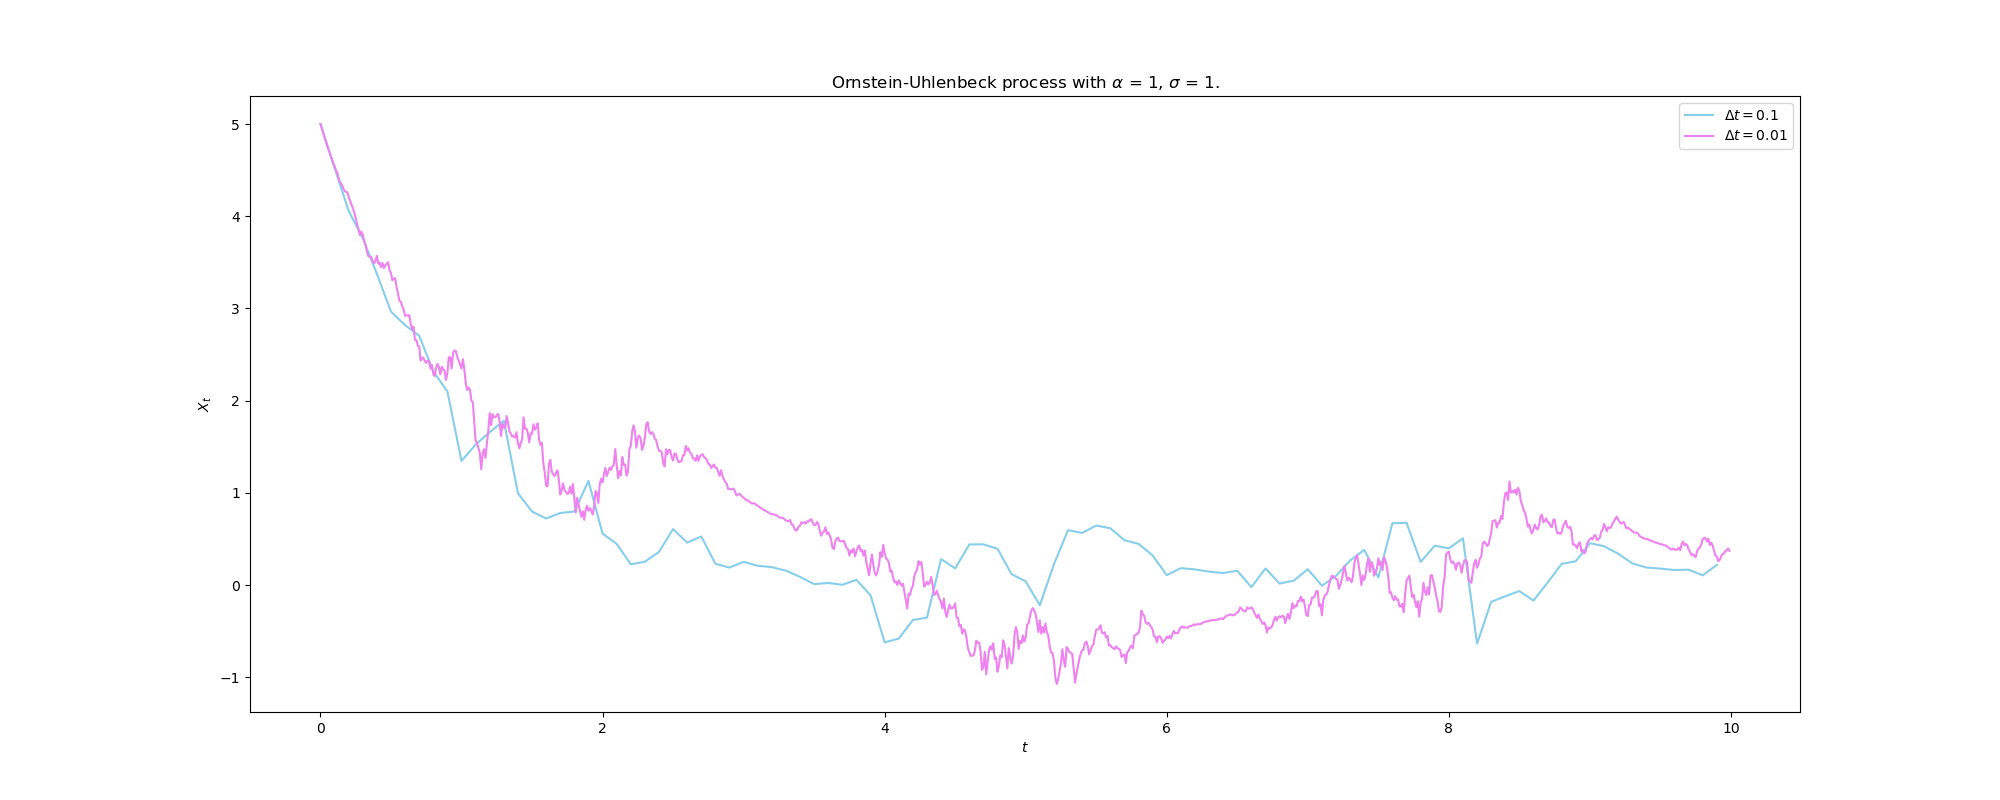
\includegraphics[width=18cm]{Ornstein_Uhlenbeck.png}
        \caption{Ornstein-Uhlenbeck Process with $\alpha = 1$, $\sigma^2 = 1$, $x_0 = 5$}
        \label{fig2}
    \end{figure}
\end{enumerate}
